%!TEX root = ../thesis.tex
%*******************************************************************************
%*********************************** First Chapter *****************************
%*******************************************************************************

\chapter{Validation Test and Preliminary Results}  %Title of the First Chapter

\ifpdf
    \graphicspath{{Chapter4/Figs/Raster/}{Chapter4/Figs/PDF/}{Chapter4/Figs/}}
\else
    \graphicspath{{Chapter4/Figs/Vector/}{Chapter4/Figs/}}
\fi

\label{chapter 4}


%**************************************************************************
In this chapter, we conduct several tests to validate the methods discussed above. The tests include the Orszag-Tang test, which validates the MHD solver and divergence cleaning; shock diffraction over a wedge/cylinder for rigid body geometries; and rotated Sod/Brio-Wu tests for outside rigid body and MHD boundary conditions.
\section{Orszag-Tang Test}
In our study, we have employed an MHD-HLLC MHD solver. To achieve second-order accuracy, the MUSCL-Hancock method has been utilized. Furthermore, to ensure the magnetic field remains divergence-free, a mixed hyperbolic/parabolic GLM divergence cleaning method has been applied. These are discussed in Chapter 3. We are using the Orszag-Tang test to validate these methods. The initial data of Orszag-Tang test is given in the Table \ref{tab:OrszagTangInitial}. The Orszag-Tang test is conducted within a spatial domain of $[0,1] \times [0,1]$ with a resolution of $256 \times 256$, employing periodic boundaries surrounding the domain. Results are analyzed at $t=0.5s$ and $t=1.0s$, under the conditions of ideal plasma with $\gamma = 5/3$. The results, depicted in Figures \ref{fig:OT}, align closely with those in Vides \textit{et al.} \cite{vides2013divergence}. However, certain discrepancies remain. These can primarily be attributed to differences in the MHD solvers utilized. Specifically, our solver employs the MHD-HLLC method, whereas Vides \textit{et al.} use the HLLD solver. This variation in methodology could account for the observed differences in results. Miki \textit{et al.} also use MHD-HLLC solver on conducting Orszag-Tang test shown on the right in Figure \ref{fig:OTComparing}. Our result is similar to theirs which validate our MHD-HLLC solver. We have The application of mixed divergence cleaning reduces diffusion and error spread significantly, as demonstrated in Figure \ref{fig13:OrszagtangDiv}. The divergence range is reduced from  [-25,30] to [-5,4].
\begin{table}[H]
\caption{Initial data for the Orszag-Tang test. }
\label{tab:OrszagTangInitial}
\centering 
\begin{tabularx}{0.8\textwidth}{@{}cccccccc@{}}
\toprule
$\rho$ & $v_x$ & $v_y$ & $v_z$  & $B_x$ & $B_y$ & $B_z$ & $p$ \\
\hline
$\gamma^2$ & $-\sin(2\pi y)$ & $\sin(2\pi x)$ & 0.0 & $-\sin(2\pi y)$ & $\sin(4\pi x)$ & $0.0$ & $\gamma$ \\
\bottomrule
\end{tabularx}
\end{table}

\begin{figure}[htbp]
\centering
\begin{minipage}[OrszagTang_mine]{0.45\textwidth}
  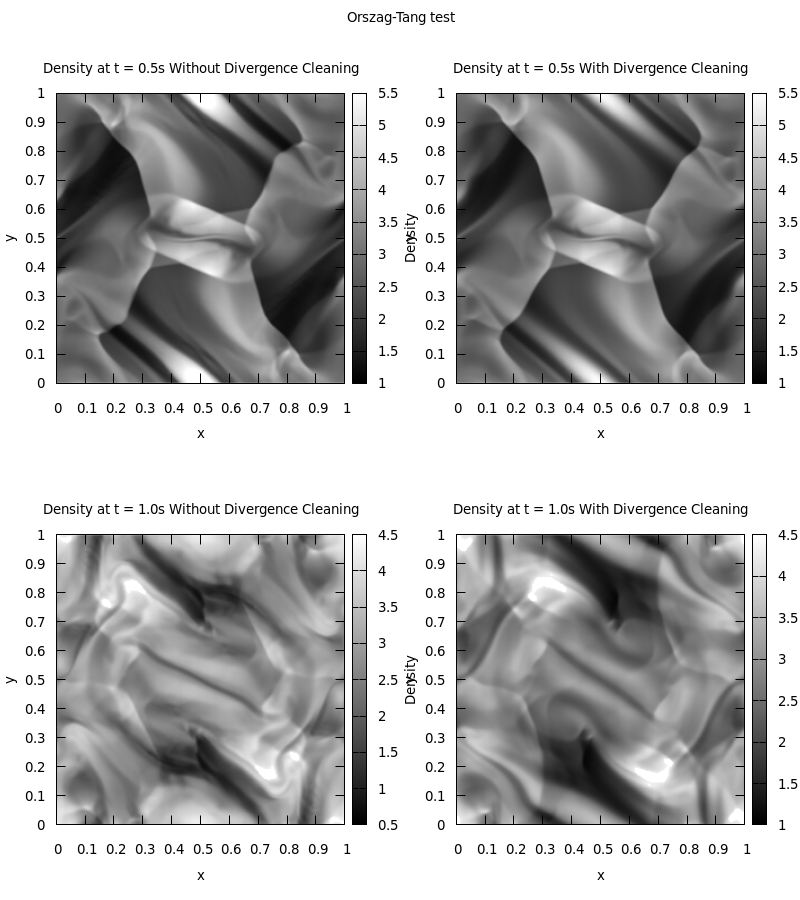
\includegraphics[width=\textwidth]{OrszagTang.png}
\end{minipage}
\begin{minipage}[OrszagTang_noDC_vides]{0.235\textwidth}
  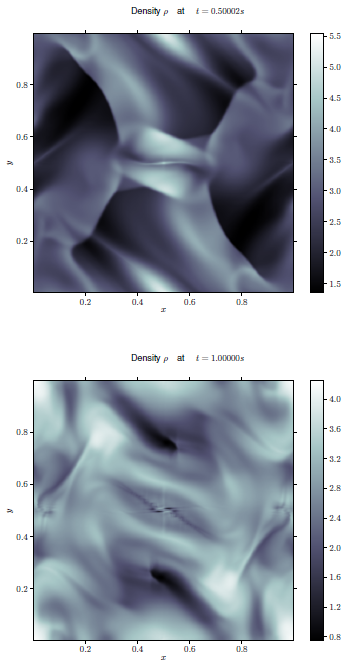
\includegraphics[width=\textwidth]{OT_no_vides.png}
\end{minipage}
\begin{minipage}[OrszagTang_yesDC_vides]{0.235\textwidth}
  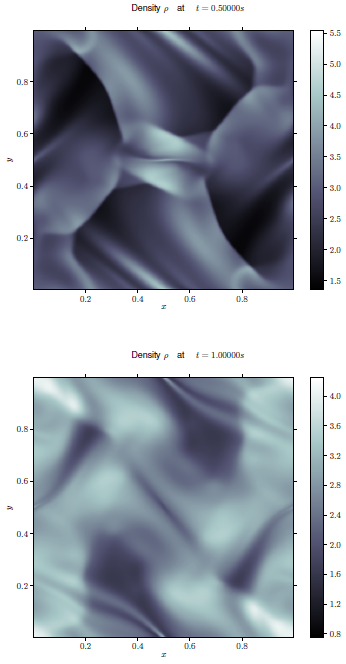
\includegraphics[width=\textwidth]{OT_yes_vides.png}
\end{minipage}
\caption[OrszagTang test]{The results of Orszag-Tang test. The left side shows our simulation results, and the right side shows the results from Vides \textit{et al.} \cite{vides2013divergence}.}
\label{fig:OT}
\end{figure}

\begin{figure}[htbp]
    \centering
    \begin{minipage}{0.45\textwidth}
  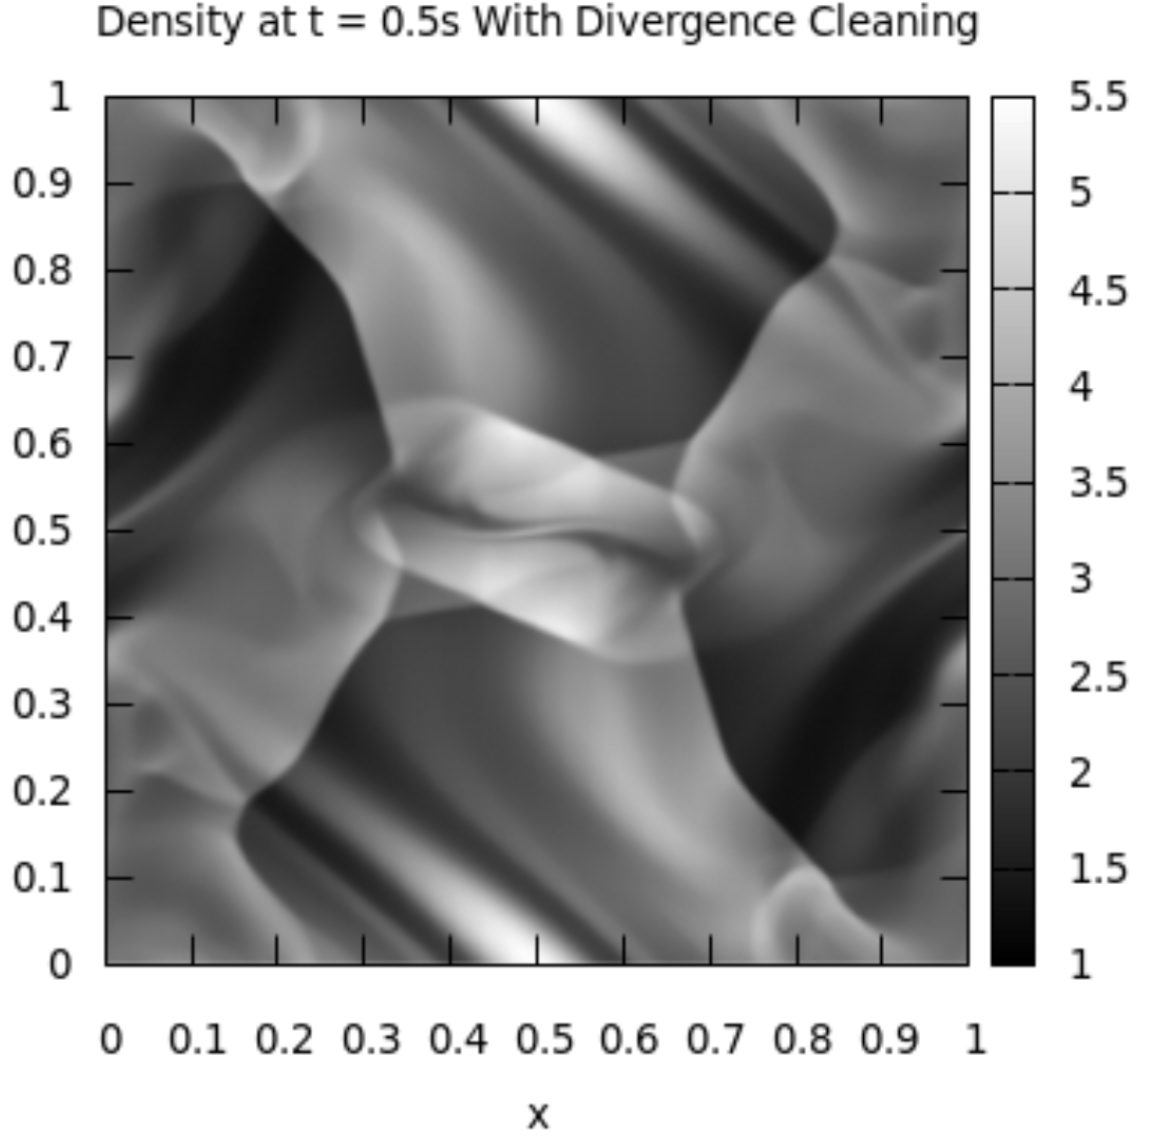
\includegraphics[width=\textwidth]{OT_mine.png}
\end{minipage}
\begin{minipage}{0.43\textwidth}
  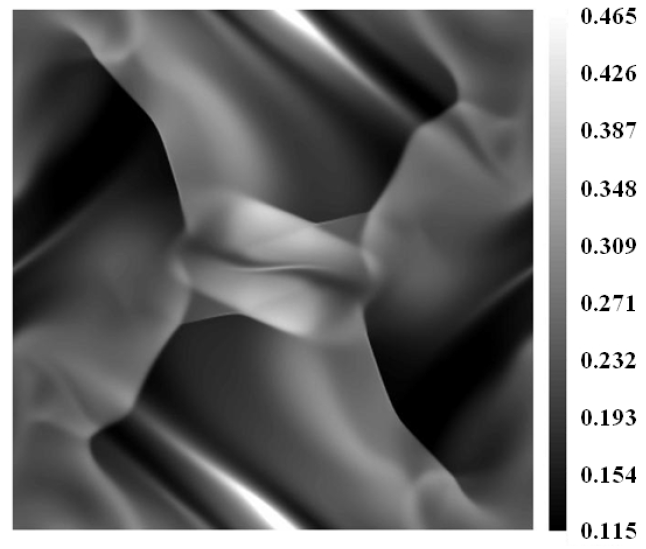
\includegraphics[width=\textwidth]{OT_Miki.png}
\end{minipage}
    \caption[Orszag-Tang with HLLC method]{Comparing the results of Orszag-Tang test with same MHD-HLLC solver. The left image shows our result produced with MHD-HLLC solver at $t=0.5$. The image on the right demonstrates the corresponding result from Miki \textit{et al.} \cite{miki2007large}. These two images look almost the same except for the different range of colorbox and resolution, which validate our MHD-HLLC method.}
    \label{fig:OTComparing}
\end{figure}

\begin{figure}[htbp]
    \centering
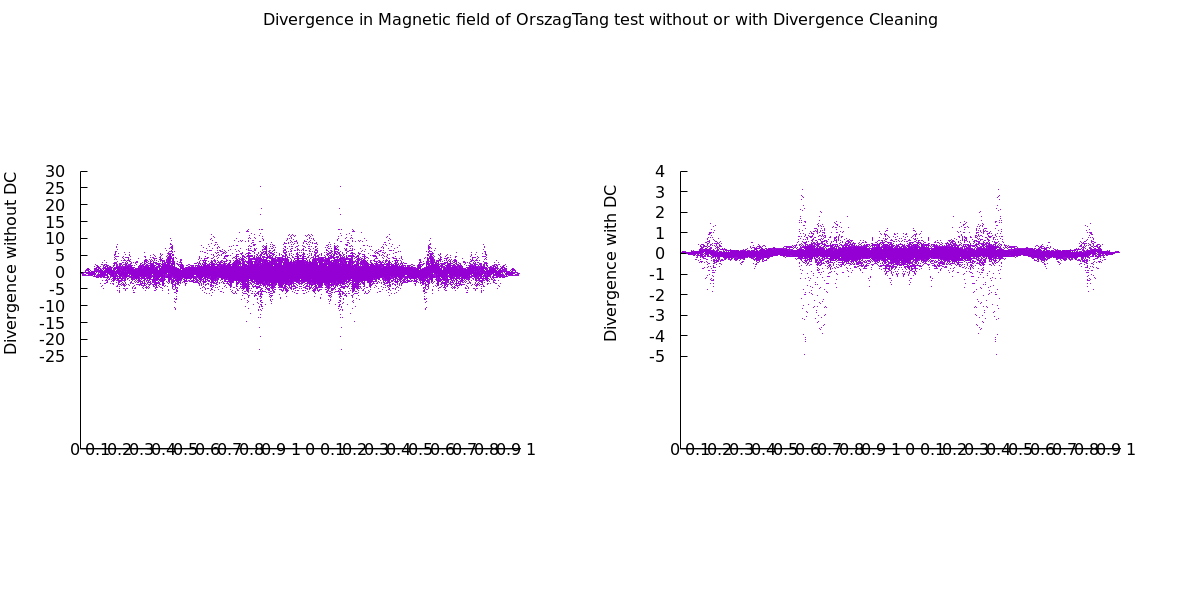
\includegraphics[width=0.9\textwidth]{OrszagTangDiv.png}
    \caption[Divergence in OrszagTang]{Divergence in the magnetic field in Orszag-Tang tests without divergence cleaning (left) and with divergence cleaning (right). These diagonal plots demonstrate the efficiency of mixed divergence cleaning. The range of divergence is reduced from [-25,30] to [-5,4]. After applying the cleaning, data points lay closer to the zero horizontal line.}
    \label{fig13:OrszagtangDiv}
\end{figure}

\begin{figure}
    \centering
    \begin{minipage}{0.46\textwidth}
  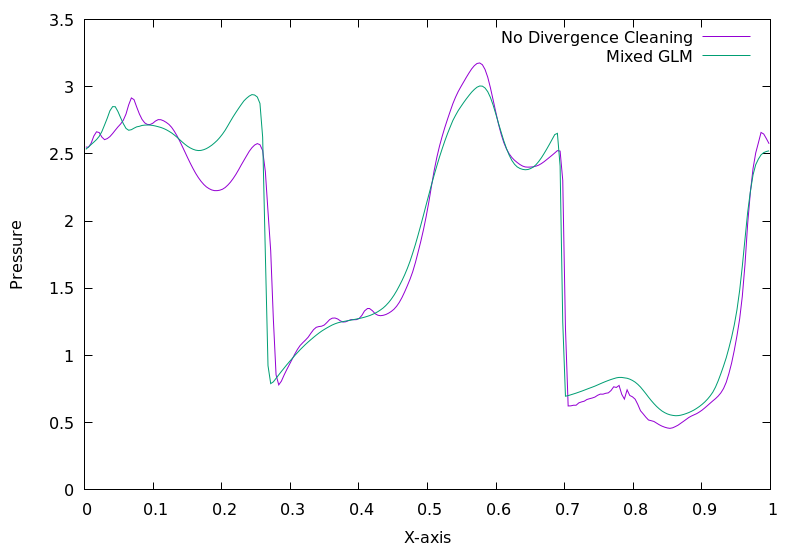
\includegraphics[width=\textwidth]{Oline.png}
\end{minipage}
\begin{minipage}{0.4\textwidth}
  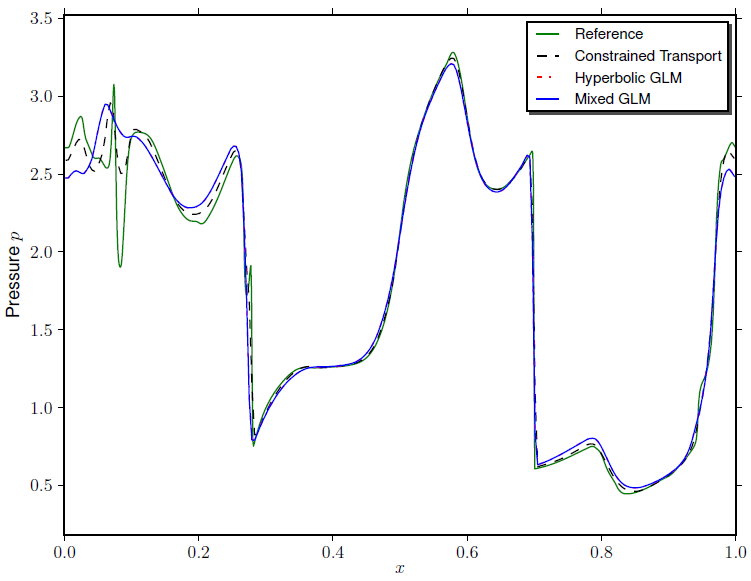
\includegraphics[width=\textwidth]{Oline_vides.png}
\end{minipage}
    \caption[OrszagTang lineout]{Horizontal lineout at $y=0.3125$ showing the gas pressure $p$ in the Orszag-Tang system at $t=0.5$. Our result (left) and Vides \textit{et al.} \cite{vides2013divergence} (right)}
    \label{fig:enter-label}
\end{figure}
\section{Shock Diffraction over Wedge}
We test a two-dimensional case where a shock with Mach number M=1.3 passes over a wedge. This test mainly validates rigid body geometries, especially for wedges and triangles geometries. The configuration is shown in Figure \ref{fig:shockwedgecon}. This shock wave satisfies the normal shock equations \cite{hernandez2018explicit} with M=1.3,   
\begin{equation*}
    \rho_s=\rho_0\frac{(\gamma+1)M^2}{2+(\gamma-1)M^2},\quad p_s=p_0\left[\frac{2\gamma M^2-(\gamma-1)}{\gamma+1}\right],\quad v_{x\_s}=\sqrt{\frac{(\rho_s-\rho_0)(p_s-p_0)}{\rho_s\rho_0}}.
\end{equation*}
We take the atmosphere as the ambient environment. A reference state is used for $\rho_{ref}=1kg/m^3$, $p_{ref}=100000Pa$, $x_{ref}=0.01m$, $v_{ref}=\sqrt{(\gamma p_{ref})/\rho_{ref}}$, $T_{ref}=x_{ref}/v_{ref}$.
Hence, a non-dimensional initial data is $p_0=1.01325$ and $\rho_0=1.225$.
The initial data is given by Table \ref{tab:shockwedge}.
\begin{table}[H]
\centering
\caption{Initial data for shock M=1.3.}
\begin{tabular}{|c|c|c|c|c|}
\hline
State & $\rho$ & $v_x$ & $v_y$ & $p$ \\
\hline
State 1 & $\rho_0$ & 0.0 & 0.0 & $p_0$\\
\hline
State 2 & $\rho_s$ & $v_{x\_s}$ & 0.0 & $p_s$\\
\hline
\end{tabular}
\label{tab:shockwedge}
\end{table}
When discontinuity for shock is set, two acoustic waves are also hidden in it. The acoustic waves affect the shock capturing. This is a well known error that arises from setting up a shock artificially \cite{LeVeque1998,Glaz1985,Hillier1995}. In our numerical simulations, we employed a methodical simplification to isolate the shockwave's effects artificially by refining the regions posterior to the shockwave by setting up the variables just as right behind the shock. This approach was implemented to ensure that the simulations focused exclusively on the propagation and characteristics of the shockwave, minimizing the influence of subsequent disturbances or secondary waves. A resolution of computational domain is $1840\times912$. The results are shown in Figure \ref{fig:shockwedge} and \ref{fig:shockwedge_con} where the figures on the left are taken from \cite{sivier1992vorticity} and correspond to an experiment done by Schardin \cite{schardin1966stossrohre}. In the simulation, oscillations are observed around the sharp angles of the wedge. These perturbations are likely attributable to the numerical challenges associated with modeling sharp geometries. Sharp corners often induce high gradient regions in the flow field, which can lead to numerical instabilities or discrepancies due to insufficient resolution or the inherent limitations of the numerical scheme employed. Enhanced mesh refinement or the implementation of more sophisticated numerical techniques may be required to accurately capture the flow dynamics in these regions.
\begin{figure}
    \centering
    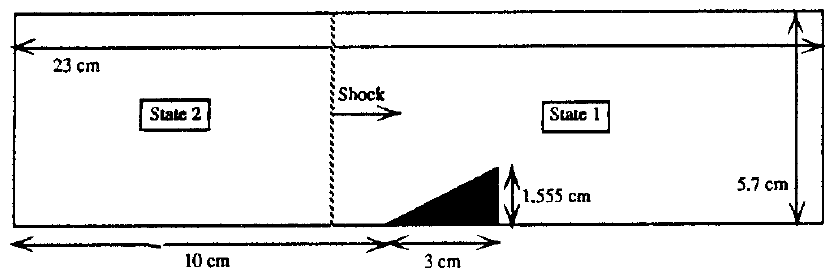
\includegraphics[width=0.9\linewidth]{shockWedgeCon.png}
    \caption[Configuration of Shock Wave and Wedge]{The computational domain configuration in the test of shock wave over a wedge. This plot is adopted from \cite{sivier1992vorticity}.}
    \label{fig:shockwedgecon}
\end{figure}

\begin{figure}
    \centering

\begin{minipage}{0.49\textwidth}
  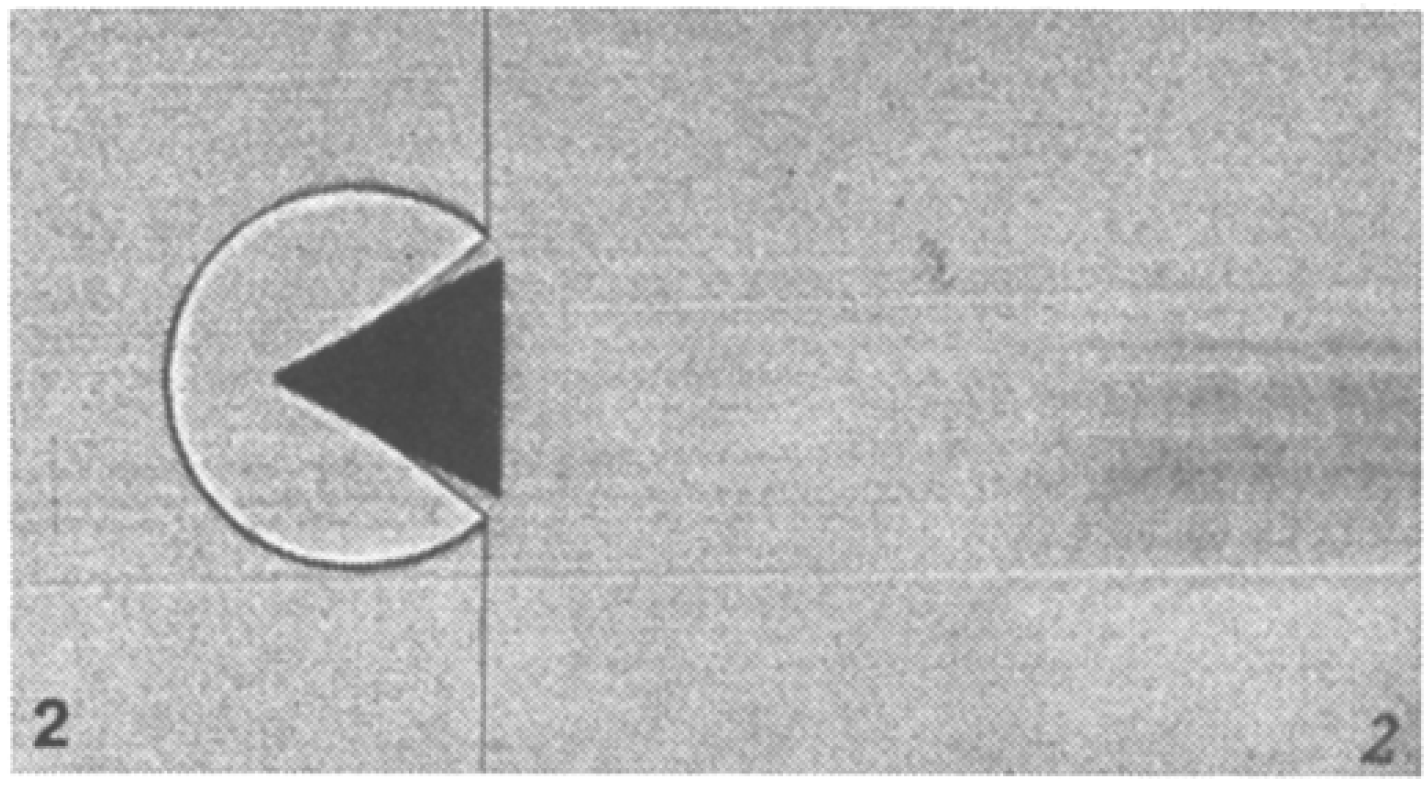
\includegraphics[width=\textwidth]{ShWe1.png}
\end{minipage}
\begin{minipage}{0.49\textwidth}
  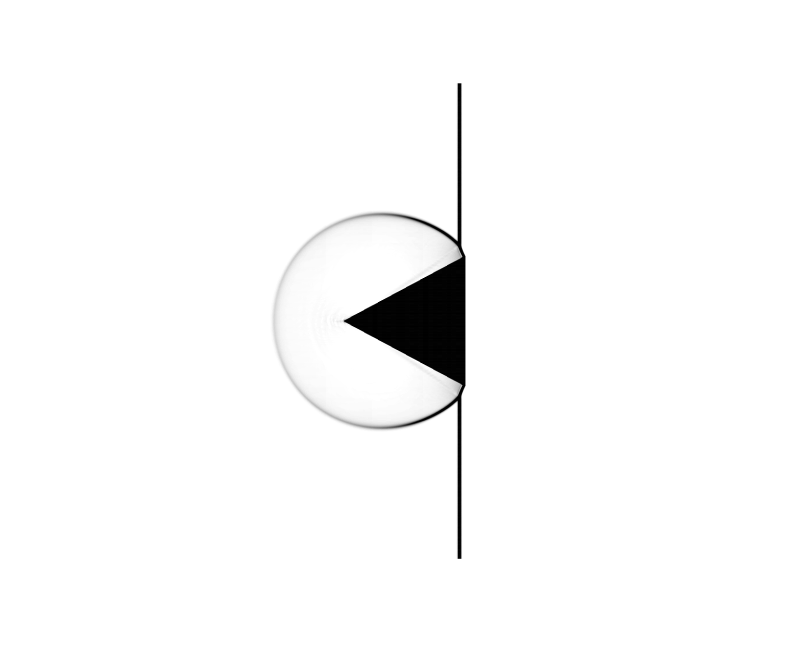
\includegraphics[width=\textwidth]{shock_wedge_2x_270.png}
\end{minipage}
\vspace{-10mm}

\begin{minipage}{0.49\textwidth}
  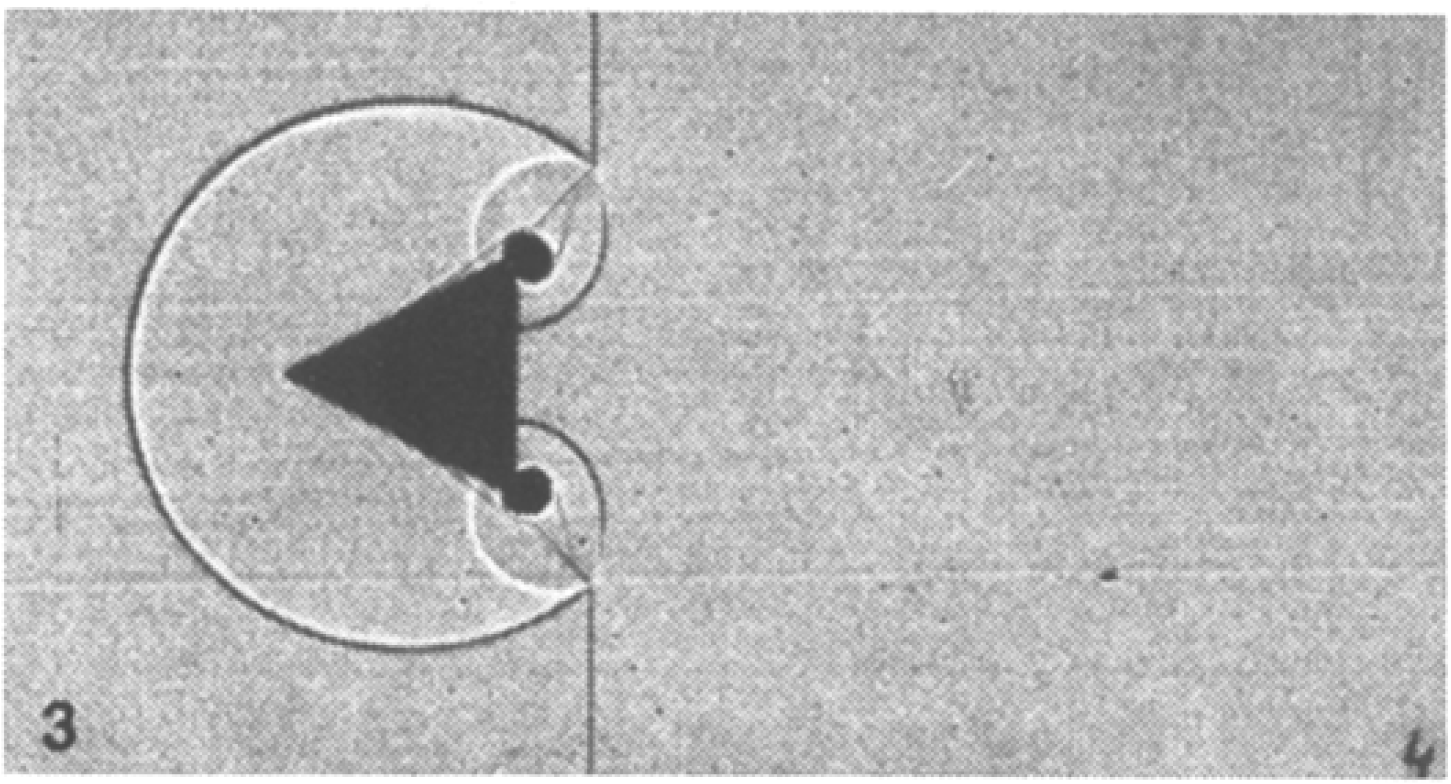
\includegraphics[width=\textwidth]{ShWe2.png}
\end{minipage}
\begin{minipage}{0.49\textwidth}
  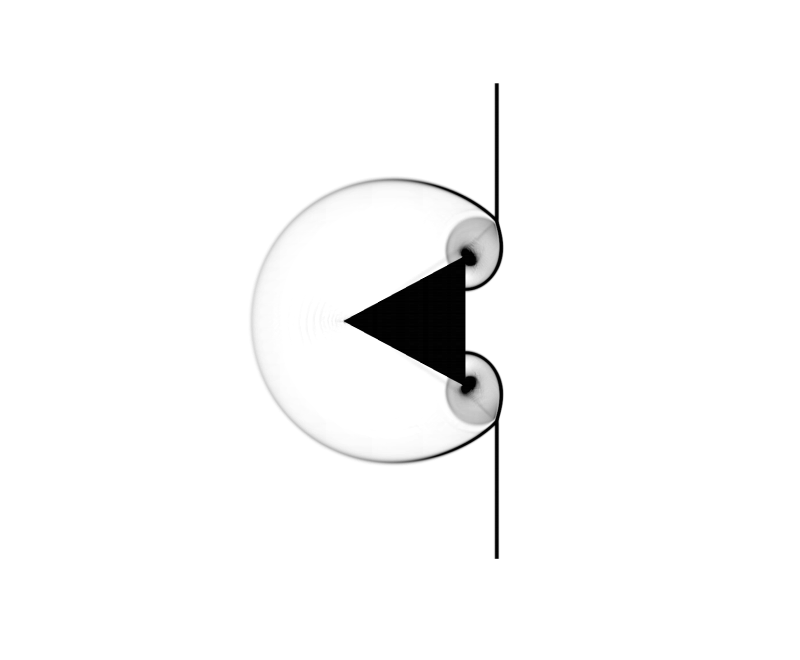
\includegraphics[width=\textwidth]{shock_wedge_2x_340.png}
\end{minipage}
\vspace{-10mm}

\begin{minipage}{0.49\textwidth}
  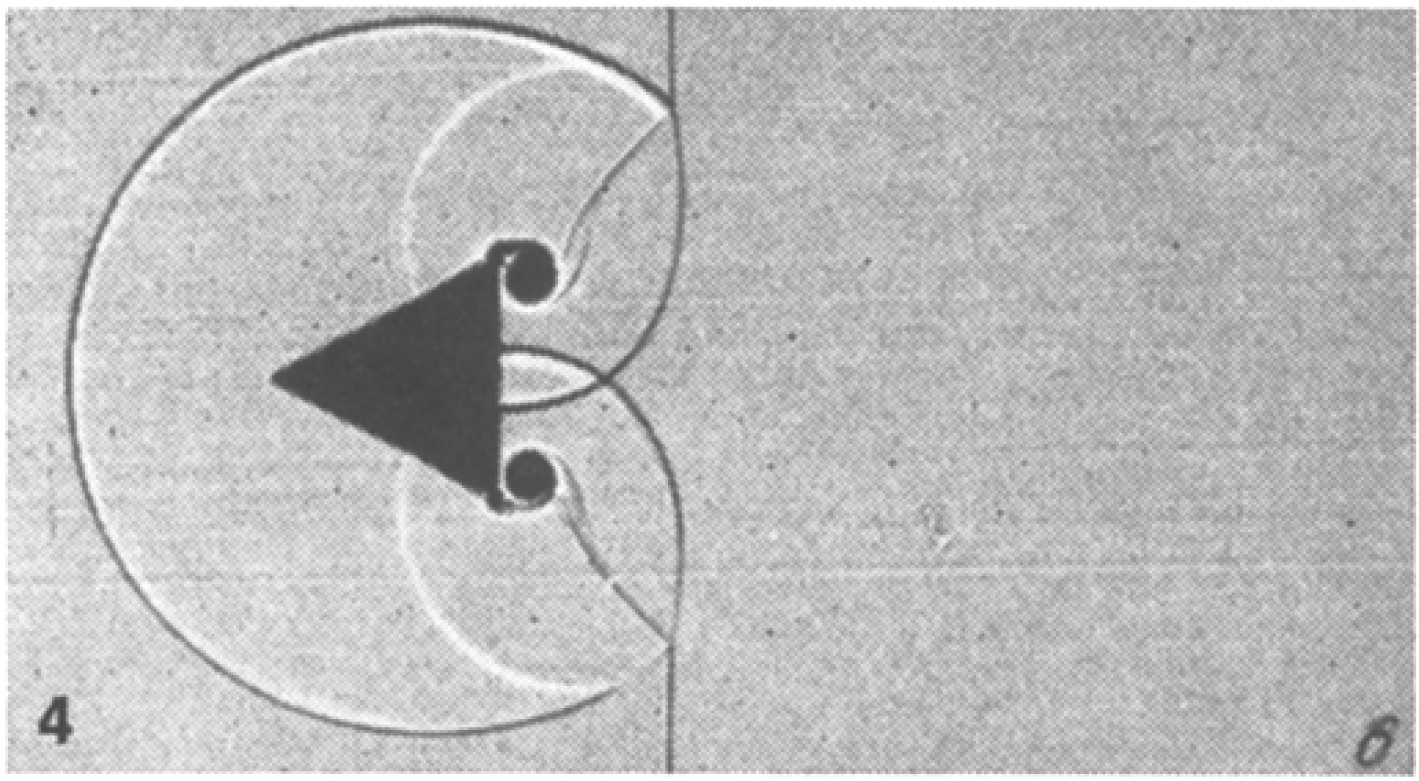
\includegraphics[width=\textwidth]{ShWe3.png}
\end{minipage}
\begin{minipage}{0.49\textwidth}
  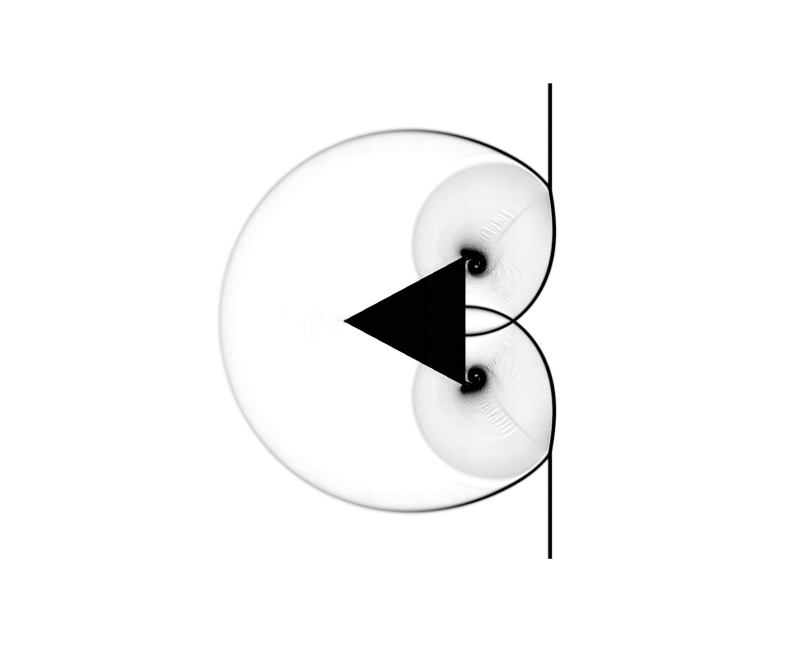
\includegraphics[width=\textwidth]{shock_wedge_2x_440.png}
\end{minipage}
\vspace{-10mm}

\begin{minipage}{0.49\textwidth}
  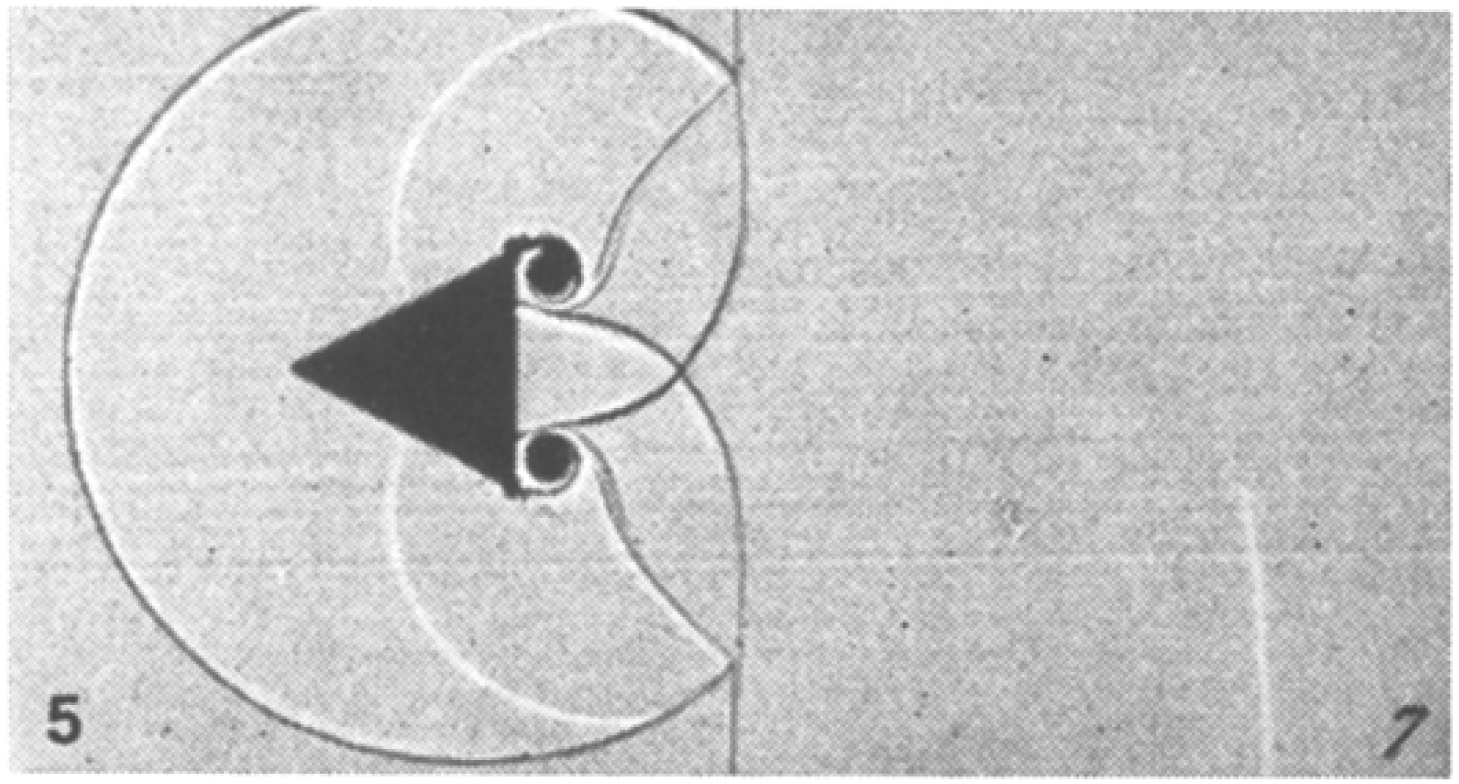
\includegraphics[width=\textwidth]{ShWe4.png}
\end{minipage}
\begin{minipage}{0.49\textwidth}
  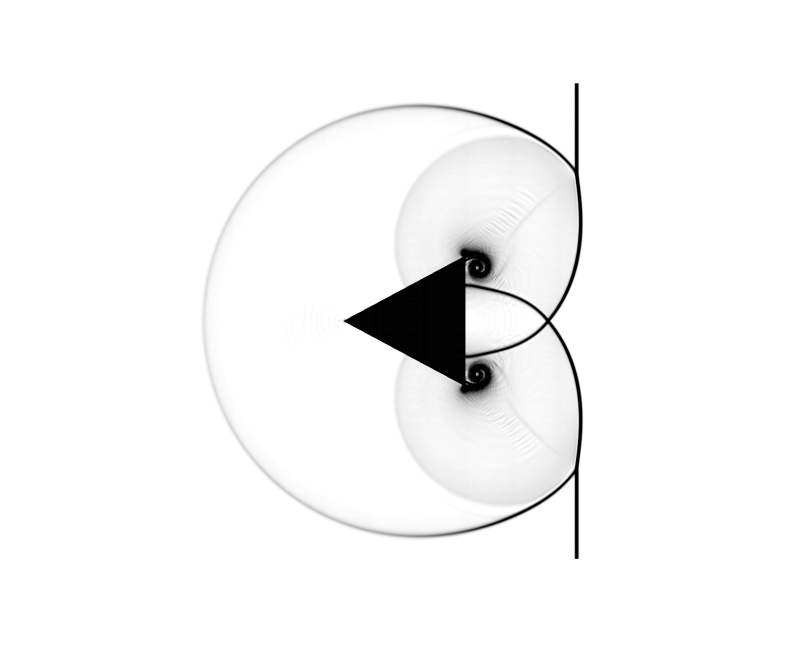
\includegraphics[width=\textwidth]{shock_wedge_2x_490.png}
\end{minipage}

    \caption[Shock diffraction over wedge]{Schlieren plots for Shock M=1.3 diffraction over wedge. The right-hand-side shows the result from simulation. Plots on the left are taken from study \cite{sivier1992vorticity} corresponding to the experiment done by Schardin \cite{schardin1966stossrohre}.}
    \label{fig:shockwedge}
\end{figure}

\begin{figure}

\begin{minipage}{0.49\textwidth}
  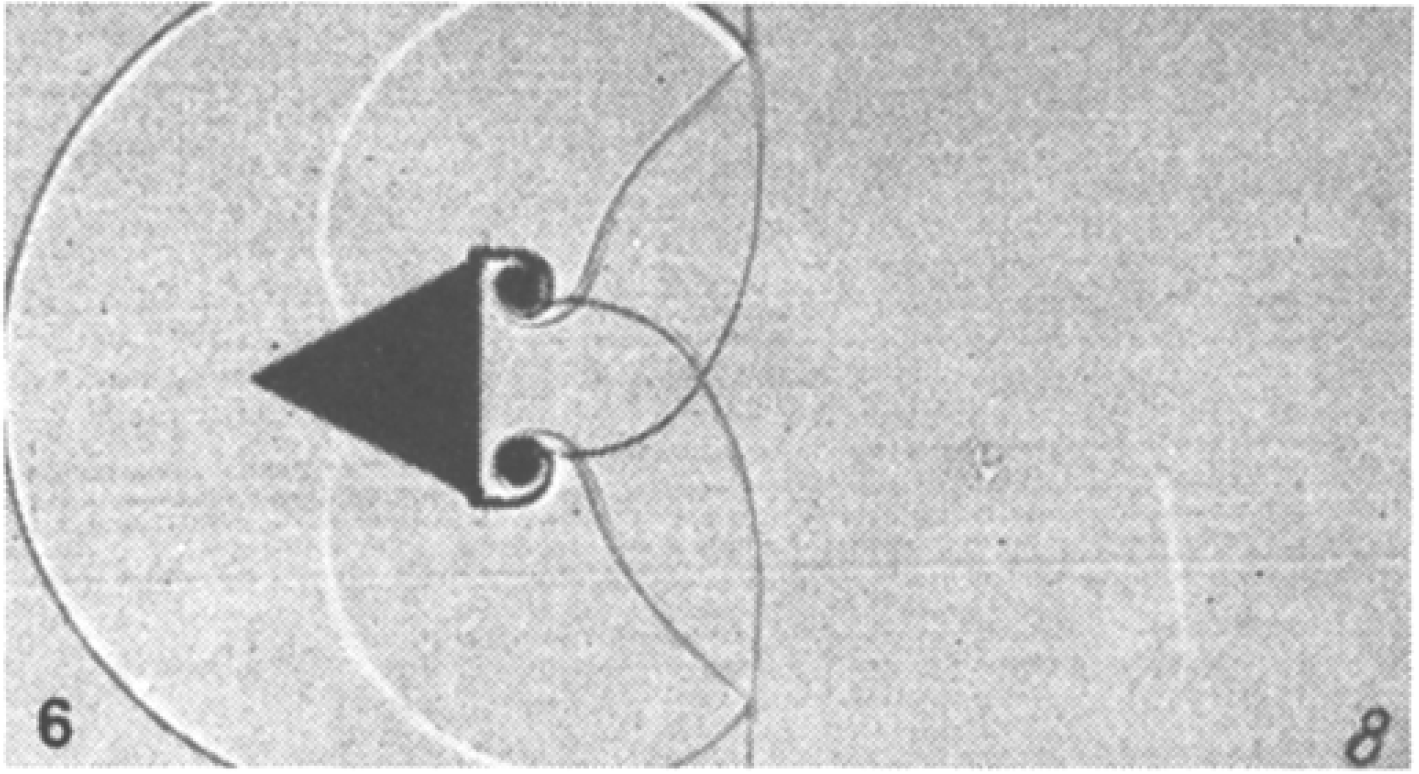
\includegraphics[width=\textwidth]{ShWe5.png}
\end{minipage}
\begin{minipage}{0.49\textwidth}
  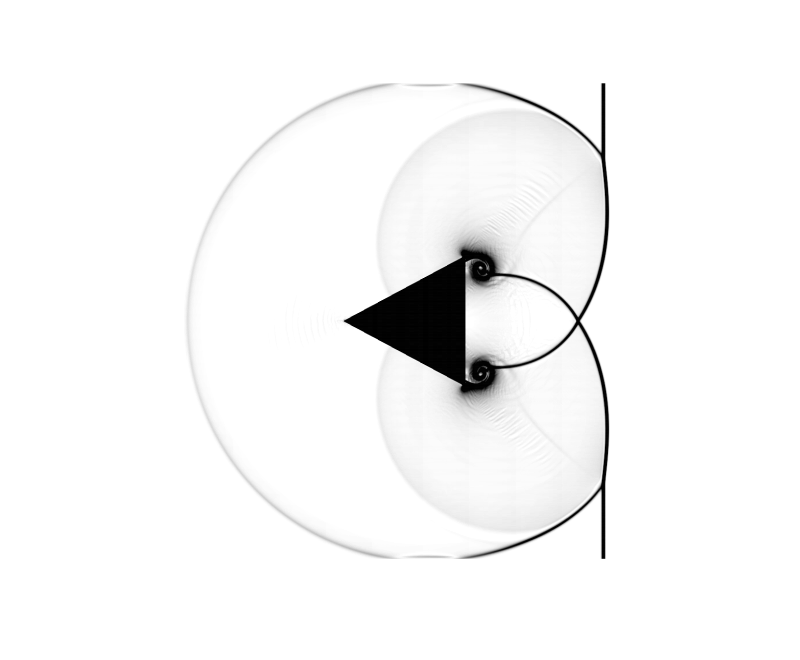
\includegraphics[width=\textwidth]{shock_wedge_2x_540.png}
\end{minipage}
\vspace{-10mm}

\begin{minipage}{0.49\textwidth}
  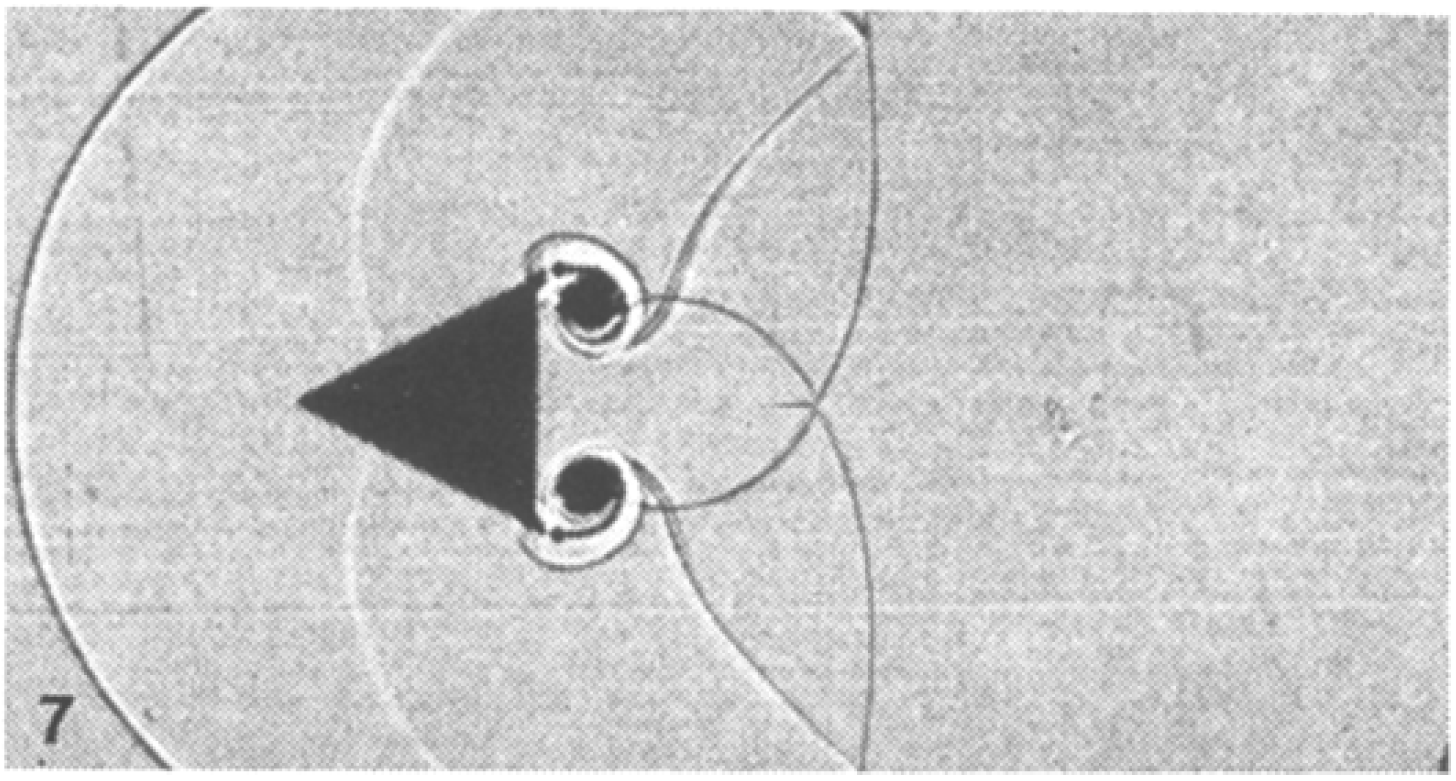
\includegraphics[width=\textwidth]{ShWe6.png}
\end{minipage}
\begin{minipage}{0.49\textwidth}
  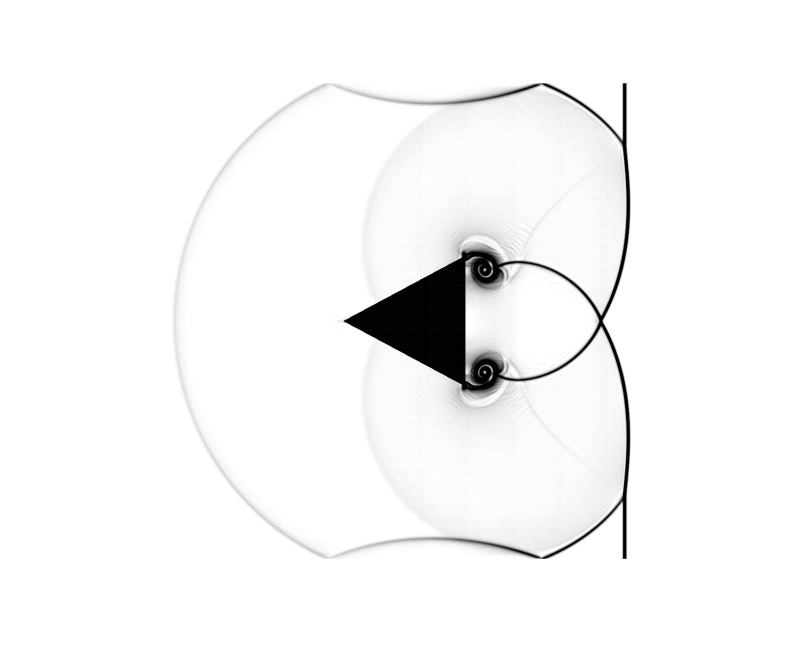
\includegraphics[width=\textwidth]{shock_wedge_2x_580.png}
\end{minipage}
\vspace{-10mm}

\begin{minipage}{0.49\textwidth}
  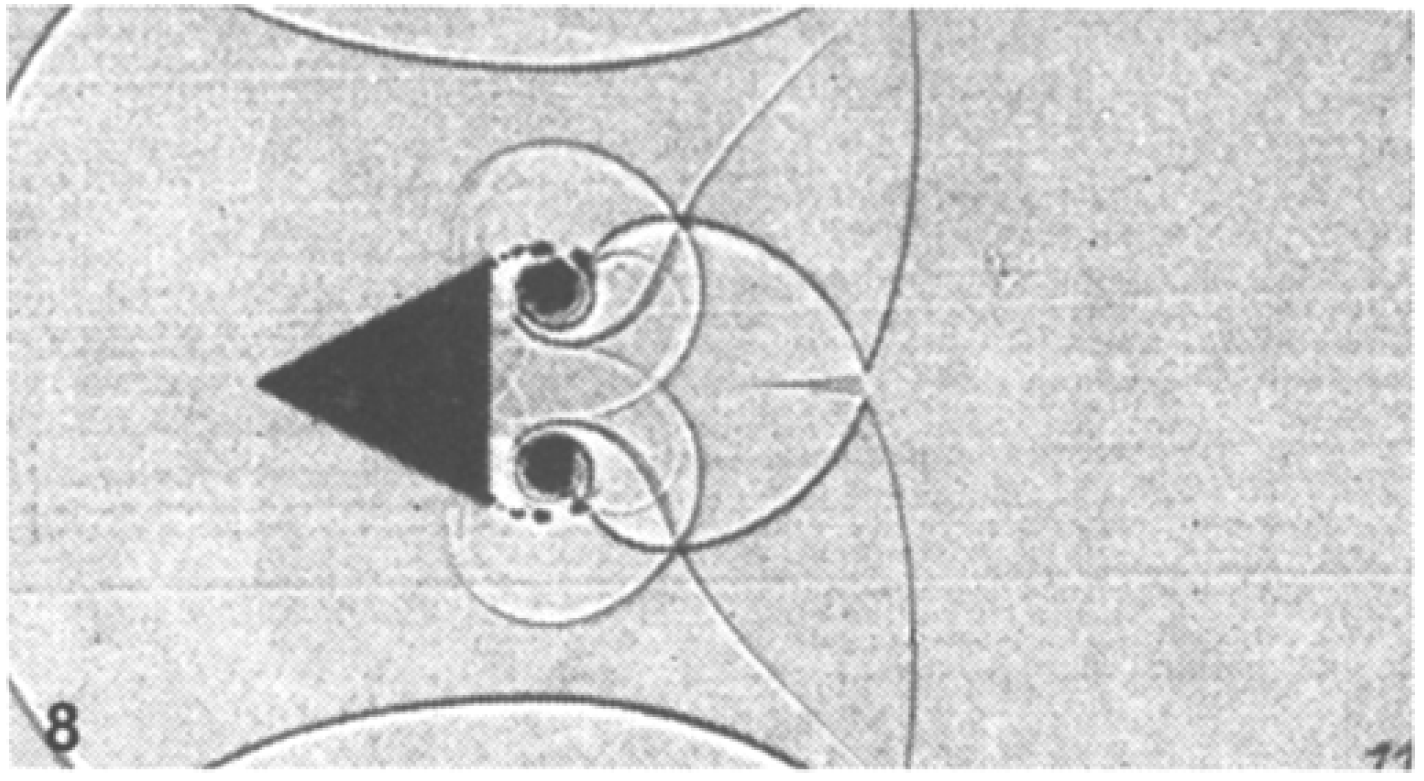
\includegraphics[width=\textwidth]{ShWe7.png}
\end{minipage}
\begin{minipage}{0.49\textwidth}
  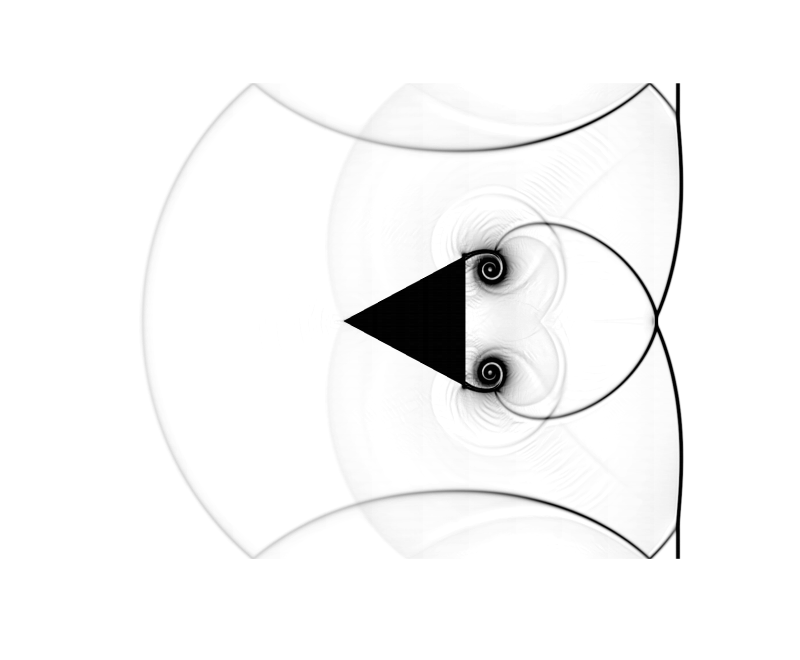
\includegraphics[width=\textwidth]{shock_wedge_2x_680.png}
\end{minipage}

\caption[Shock diffraction over wedge continuing]{Continue plots of Figure \ref{fig:shockwedge}}
    \label{fig:shockwedge_con}

\end{figure}

\section{Shock Diffraction over Cylinder}
A similar two-dimensional case is tested for cylinder with shock M=2.81, using the same normal shock equations and ambient environment, with the same reference states and non-dimensional initial values $\rho_0=1.225$ and $p_0=1.01325$. This test validates circle geometries for rigid bodies. In this test, a similar artificial shock is used. The computational domain is $[0,4]\times[-2,2]$ with $800\times800$ resolution. A circle representing a planar cylinder is set at the center $(2,0)$ with a radius of 0.5. The result is demonstrated in Figure \ref{fig:ShockCy}. The left density image is adopted from \cite{bryson1961diffraction}.

\begin{figure}[htbp]
\centering
\begin{minipage}{0.25\textwidth}
  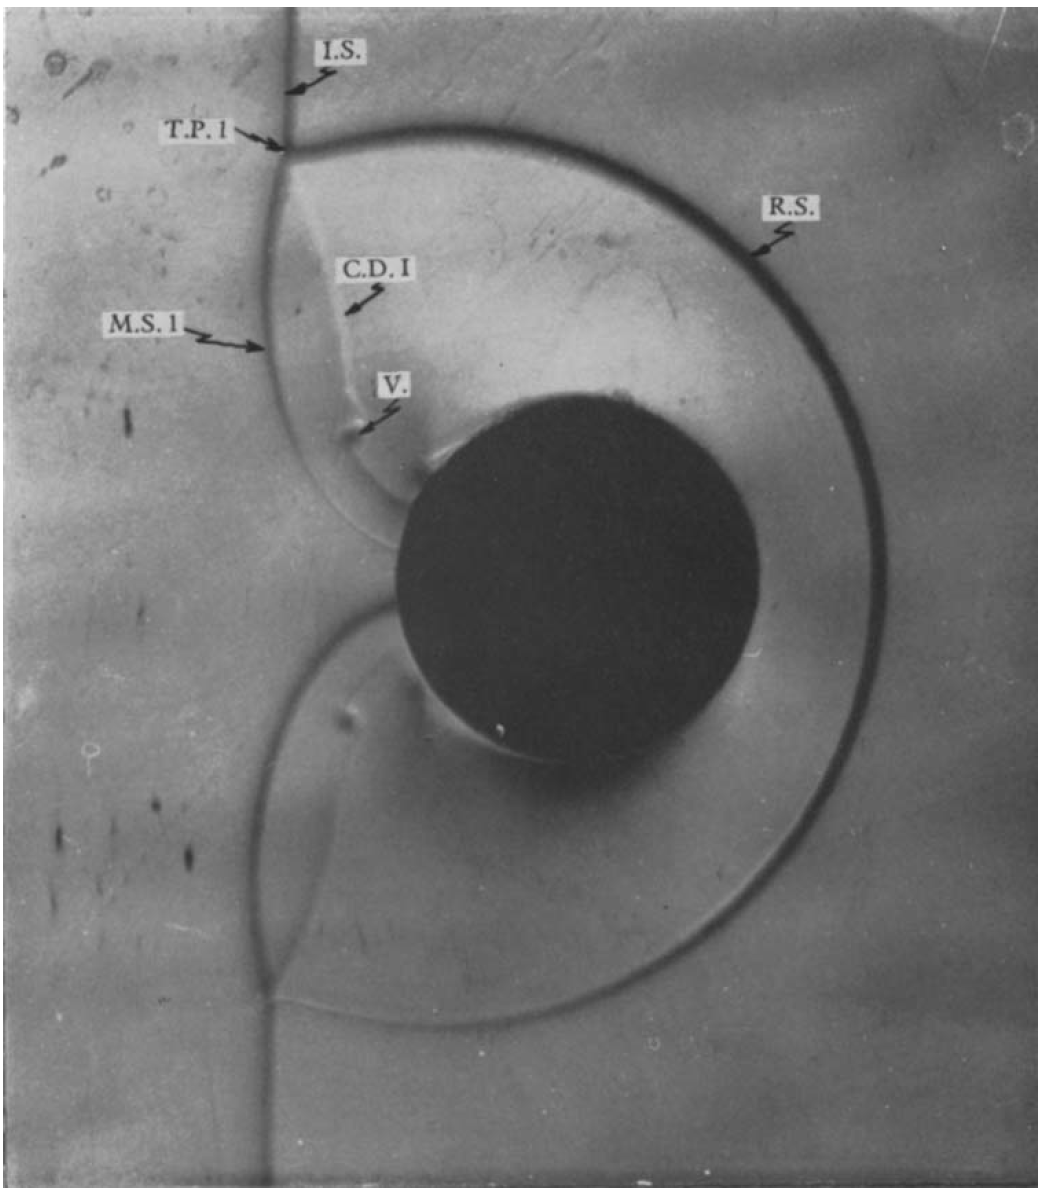
\includegraphics[width=\textwidth]{ShCy.png}
\end{minipage}
\begin{minipage}{0.45\textwidth}
  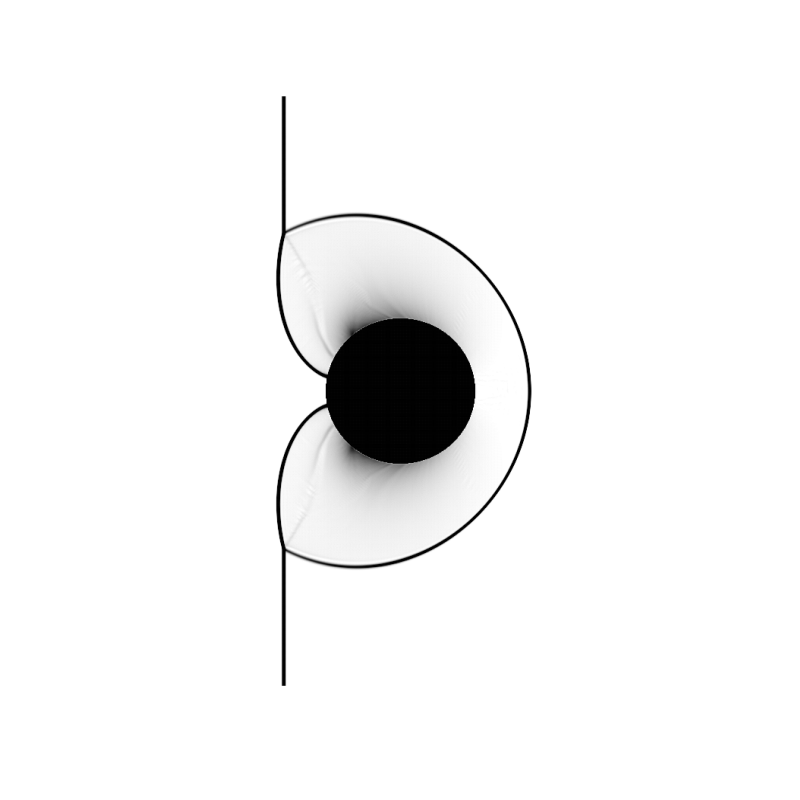
\includegraphics[width=\textwidth]{shock_cylinder_95.png}
\end{minipage}
\caption[Shock diffraction over cylinder]{Schlieren plots for Shock M=2.81 diffraction over a cylinder. The right-hand side shows the result from simulation compared with the image on the left demonstrating the corresponding experiment done by Bryson \cite{bryson1961diffraction}.}
\label{fig:ShockCy}
\end{figure}

\section{Tests in Rotated Rigid Body}
\subsection{Rotated Sod Test}
On the fixed rigid body, we apply a reflective boundary condition, where no-penetration condition and slip condition are used for normal and tangential velocities, respectively. A one-dimensional test is applied to validate the performance of these boundary conditions under the Euler system. 
\begin{figure}[htbp!]
    \centering
    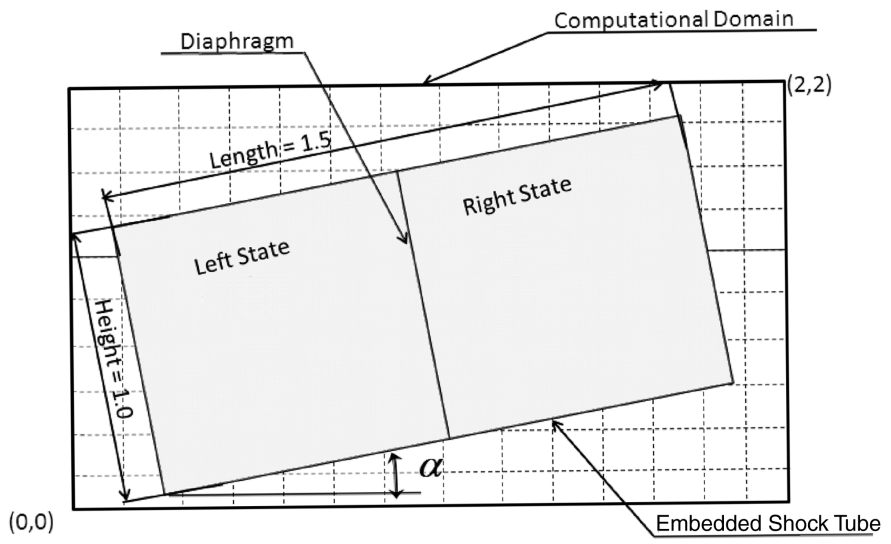
\includegraphics[width=0.5\linewidth]{tube.png}
    \caption[Rotated Tube]{A demonstration of the computational domain and the fixed tube in it. The tube is centered at $(1,1)$ and rotated by an angle $\alpha$. Our tests are mainly conducted within this tube. This plot is adopted from Sambasvian \textit{et al.} \cite{sambasivan2009ghost}.}
    \label{fig:tube}
\end{figure}
As shown in Figure \ref{fig:tube}, we use a computational area of $[0,2]\times[0,2]$ with a resolution $300\times300$, where a rectangle tube is set in this domain with a length of 1.5 and a width of 1.0. The tube is rotated at different angles $\alpha=30^\circ$, $\alpha=45^\circ$, $\alpha=60^\circ$ for throughout testing. The computational test we use is a variant of the Sod test from Toro \textit{et al.} \cite{toro2013riemann}, where the initial states are given in table \ref{tab:sod}.
\begin{table}[H]
\centering
\caption[Sod test]{Initial states for Sod test.}
\begin{tabular}{|c|c|c|c|c|}
\hline
State & $\rho$ & $p$ & $v_x$ & $v_y$ \\
\hline
Left state & 1.0 & 1.0 & 0.0 & 0.0 \\
\hline
Right state & 0.125 & 0.1 & 0.0 & 0.0 \\
\hline
\end{tabular}
\label{tab:sod}
\end{table}
The discontinuity is set in the middle length of the tube. The simulation is carried out to $T=0.25$. We lineout the results in the middle width.  Their densities are demonstrated in lineout Figure \ref{fig:rotateSod} along with the exact solutions and heat Figure \ref{fig:rotateSod_heat}. The results show good agreement with the exact solutions.


  \begin{figure}
      \centering
      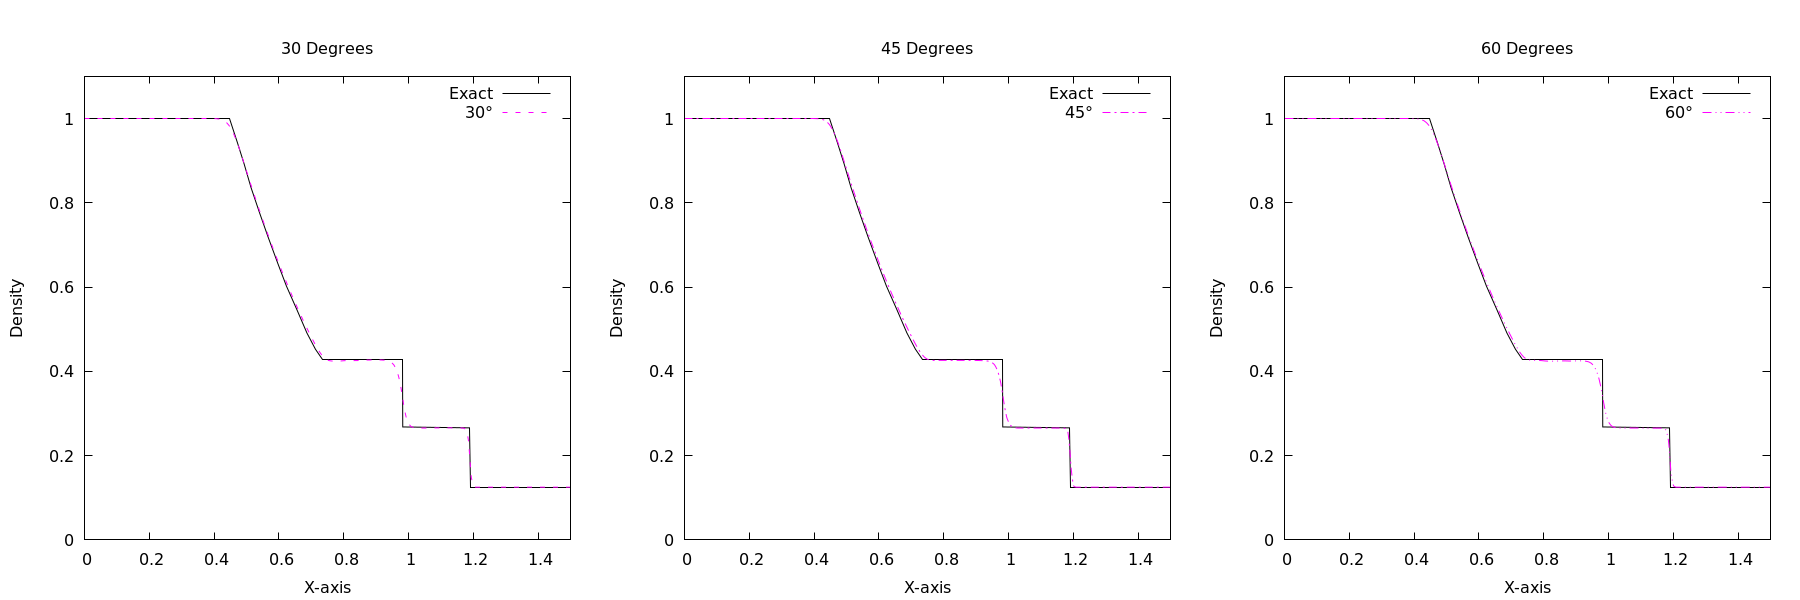
\includegraphics[width=1\linewidth]{rotateSod.png}
      \caption[Lineout for rotated Sod test]{The results of Sod test in a rotated tube with exact solutions. The rotated angles are $\alpha=30^\circ$ (left), $\alpha=45^\circ$ (middle), $\alpha=60^\circ$ (right). Results agree with the exact solutions.}
      \label{fig:rotateSod}
  \end{figure}
  \begin{figure}
      \centering
      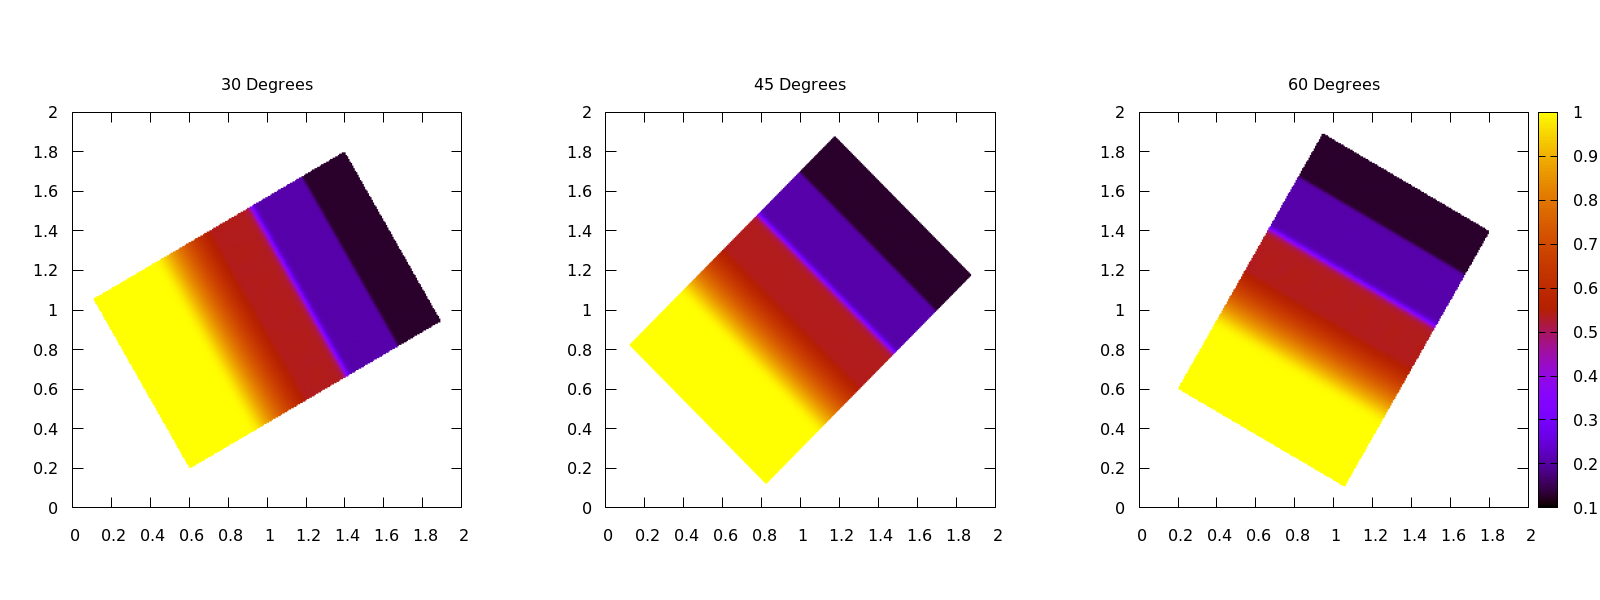
\includegraphics[width=1\linewidth]{rotateSod_heat.png}
      \caption[Heat plot for rotated Sod test]{A heat plot for rotated Sod test showing the tests at different angles.}
      \label{fig:rotateSod_heat}
  \end{figure}
  
\subsection{Rotated Brio-Wu Test}
  The rigid body is regarded as a perfect conductor in validation. A similar 'no-penetration' condition for the normal magnetic field and 'slip' condition for tangential magnetic field are applied. We use the Brio-Wu test \cite{brio1988upwind} to validate these conditions. A similar shock tube is set as shown in Figure \ref{fig:tube}. The Brio-Wu test have a similar initial data to the Sod test but with a non-zero magnetic field and $\gamma=2.0$. Compared with the original test, we adjust the magnetic variables to fit them in the tube. The states for this test are given in Table \ref{tab:Brio}.
  \begin{table}[H]
\centering
\caption[Rotated Brio-Wu test]{Initial states for the rotated Brio-Wu test. $\alpha$ is the rotation angle.}
\begin{tabular}{|c|c|c|c|c|c|c|c|c|}
\hline
State & $\rho$ & $p$ & $v_x$ & $v_y$ & $v_z$ & $B_x$ & $B_y$ & $B_z$ \\
\hline
Left state & 1.0 & 1.0 & 0.0 & 0.0 & 0.0 & $0.75*cos(\alpha)$ & $0.75*sin(\alpha)$ & 1.0 \\
\hline
Right state & 0.125 & 0.1 & 0.0 & 0.0 & 0.0 & $0.75*cos(\alpha)$ & $0.75*sin(\alpha)$ & -1.0\\
\hline
\end{tabular}
\label{tab:Brio}
\end{table}
  A perfect conducting wall condition is applied around the boundary of this tube. We set the initial magnetic field with same normal component as in Table \ref{tab:Brio} with Dirichlet conditions. We reflect the normal magnetic changes on boundary for a 'no-penetration' condition. Such boundary condition stabilize the magnetic field in the shock tube. The simulation is carried out to $T=0.1$. The results are shown in lineout Figure \ref{fig:rotateBrioWu} and heat Figure \ref{fig:rotateBrioWu_heat}. They are similar to the exact solution, which validate the perfect conducing condition we applied. 
  

 \begin{figure}
      \centering
      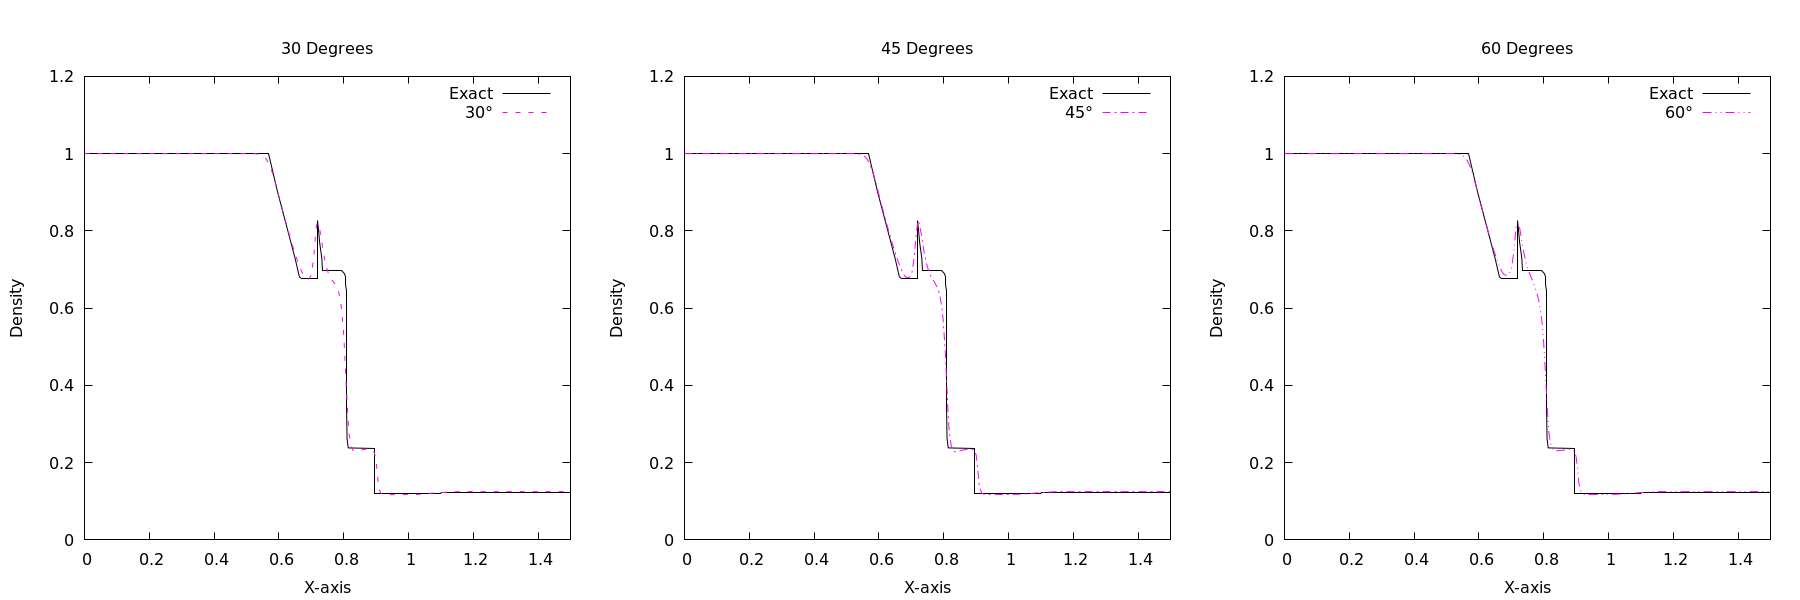
\includegraphics[width=1\linewidth]{rotateBrioWu.png}
      \caption[Lineout for rotated Brio-Wu]{The results of the rotated Brio-Wu test with exact solutions. The results are slightly different from exact solution because of the resolution, but they still validate the perfect conductor condition.}
      \label{fig:rotateBrioWu}
  \end{figure}
  \begin{figure}
      \centering
      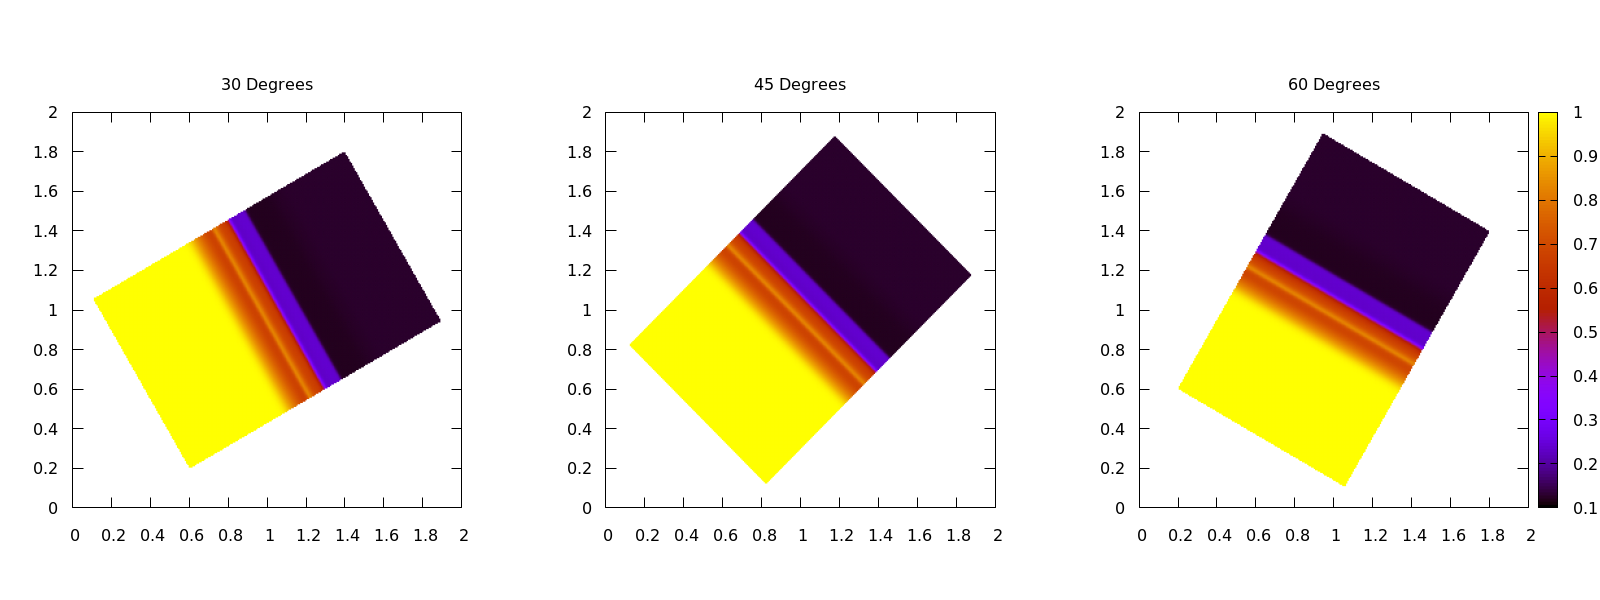
\includegraphics[width=1\linewidth]{rotateBrioWu_heat.png}
      \caption[Heat plot for rotated Brio-Wu test]{A heat plot for rotated Brio-Wu test, showing tests at different angles.}
      \label{fig:rotateBrioWu_heat}
  \end{figure}

  
